\setauthor{AC}
\section{Implementierung der Abo-Verwaltung}
Ein wesentlicher Bestandteil meines Projektteils war die Umsetzung der Benutzeroberfläche zur Verwaltung persönlicher Streaming-Abonnements. Ziel war es, eine übersichtliche und einfach bedienbare Ansicht zu entwickeln, in der Nutzende ihre aktiven Anbieter verwalten und Änderungen direkt speichern können. Die technische Umsetzung erfolgte im Angular-Frontend mit einer eigenständigen Komponente für die Providerverwaltung sowie zugehörigen Services für die Kommunikation mit dem Backend \cite{angular_overview,angular_forms}.

\subsection{Aufbau der Provider-Verwaltung}
Die Provider-Verwaltung wurde als eigener geschützter Bereich innerhalb der Angular-Anwendung umgesetzt. Nutzende können dort Streaming-Anbieter laden, durchsuchen und auswählen. Zusätzlich ist erkennbar, welche Anbieter bereits im Profil gespeichert sind. Diese Struktur verbessert die Übersichtlichkeit und ermöglicht eine klare Trennung zwischen allgemeinen Filmfunktionen und persönlichen Abo-Daten.

Technisch wurde dieser Bereich als eigenständige Frontend-Ansicht mit zugehöriger Verwaltungslogik aufgebaut. Eine zuständige Angular-Komponente übernimmt die Darstellung der Anbieterübersicht, der aktiven Filter und der Eingabefelder für Abo-Daten. Der eigentliche Datenzugriff erfolgt über Services, die beim Öffnen der Ansicht zunächst die verfügbaren Anbieter sowie die bereits gespeicherten benutzerspezifischen Abonnements laden. Auf dieser Grundlage kann das Frontend sofort sichtbar machen, welche Anbieter bereits aktiv sind und bei welchen Einträgen noch keine persönlichen Daten hinterlegt wurden.

\subsection{Bearbeitung und Speicherung von Abonnements}
In der Oberfläche können Nutzende Anbieter als aktiv markieren und zusätzliche Angaben wie Abrechnungszyklus und Datum der letzten Abbuchung festlegen. Diese Eingaben werden im Frontend verarbeitet und anschließend gesammelt an das Backend übermittelt. Die Verwendung von Formularlogik und Datenbindung in Angular erleichtert dabei die direkte Verknüpfung zwischen Eingabefeldern und angezeigten Daten \cite{angular_forms}. Dadurch konnten Änderungen in der Oberfläche unmittelbar sichtbar gemacht werden.

Für die Umsetzung bedeutete das konkret, dass Änderungen zunächst im Zustand der Komponente verarbeitet und anschließend über einen zuständigen Service an das Backend übertragen werden. Die Oberfläche muss dabei sowohl bereits gespeicherte Daten korrekt anzeigen als auch neue oder geänderte Werte übernehmen. Dadurch entsteht ein durchgängiger Ablauf aus Laden, Bearbeiten, Absenden und erneuter Anzeige der aktualisierten Daten. Gerade bei der Abo-Verwaltung war diese Logik wichtig, weil nicht nur einzelne Werte angezeigt werden, sondern Anbieterstatus, Zyklus, Datumsangaben und weitere Abo-Metadaten fachlich zusammengehören.

\begin{figure}[H]
    \centering
    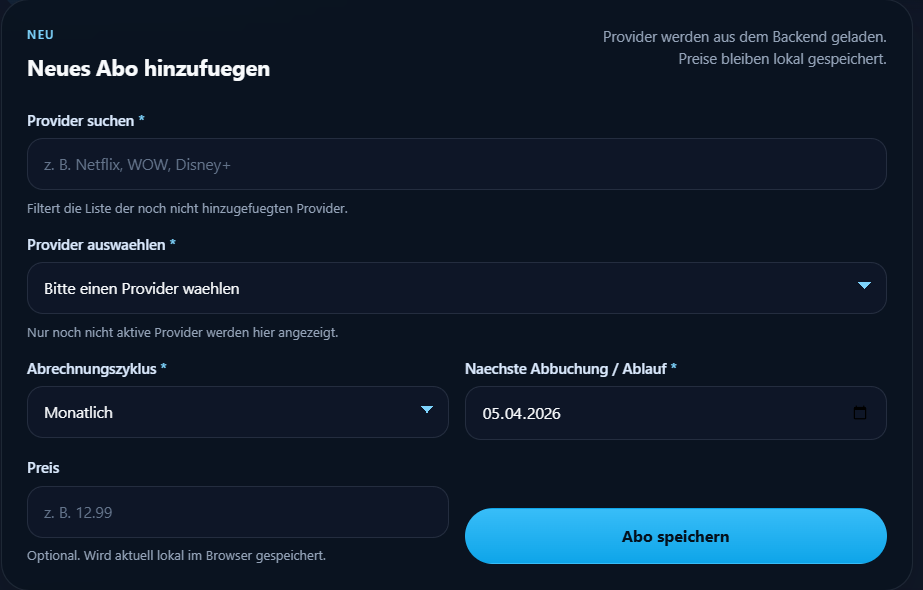
\includegraphics[width=\textwidth]{pics/6.1.2_Bild}
    \caption{Erfassungsmaske für ein Streaming-Abonnement}
    \label{fig:subscription_input_form}
\end{figure}

\subsection{Filter- und Suchfunktionen in der Oberfläche}
Damit die Verwaltung vieler Anbieter benutzerfreundlich bleibt, wurde die Oberfläche um Such- und Filterfunktionen ergänzt. Nutzende können nach Anbietern suchen oder sich nur bereits aktivierte Abonnements anzeigen lassen. Diese Interaktionsmöglichkeiten verbessern die Nutzbarkeit der Anwendung deutlich, da relevante Einträge schneller gefunden und bearbeitet werden können.

Die Such- und Filterlogik wurde direkt in der Benutzeroberfläche verarbeitet. Dazu werden geladene Anbieterlisten im Frontend anhand der aktuellen Eingaben gefiltert und anschließend in der Ansicht aktualisiert dargestellt. Dieses Vorgehen ist für den Projektkontext sinnvoll, weil die eigentlichen Abo-Daten bereits geladen sind und die Oberfläche schnell auf Änderungen reagieren soll, ohne bei jeder kleinen Filteranpassung einen neuen Request auszulösen. Die Kombination aus geladener Datenbasis, sichtbarer Markierung aktiver Abos und lokaler Suchlogik machte die Provider-Verwaltung deutlich alltagstauglicher.

\begin{figure}[H]
    \centering
    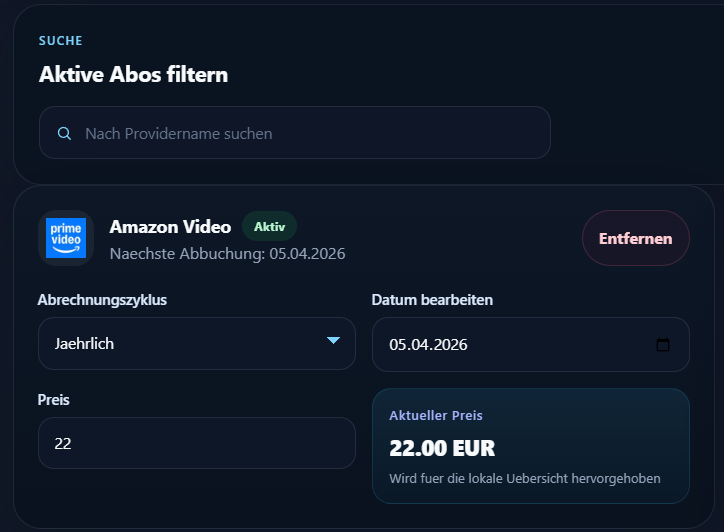
\includegraphics[width=\textwidth]{pics/Abbildung_5}
    \caption{Abo-Verwaltung mit Such-, Filter- und Bearbeitungsfunktionen}
    \label{fig:placeholder_subscription_management}
\end{figure}

\section{Darstellung von Laufzeiten und Kündigungszeitpunkten}
Neben der Auswahl von Streaming-Anbietern war auch die Darstellung zeitlicher Informationen ein wichtiger Teil der Abo-Verwaltung. Aus Frontend-Sicht ging es dabei vor allem darum, Eingabemöglichkeiten für abrechnungsrelevante Daten bereitzustellen und diese verständlich in die Oberfläche einzubinden. Nutzende sollen dadurch ihre gespeicherten Abonnements besser nachvollziehen können.

\subsection{Erfassung abrechnungsrelevanter Daten}
Für jedes aktive Abonnement können im Frontend Informationen wie Abrechnungszyklus und Datum der letzten Abbuchung erfasst werden. Diese Werte werden in Formularfeldern dargestellt und von den Nutzenden bearbeitet. Die Oberfläche unterstützt dadurch nicht nur die Auswahl eines Anbieters, sondern auch die strukturierte Verwaltung der wichtigsten Abo-Metadaten. Bereits umgesetzt ist damit die Eingabe und Speicherung jener Daten, die später als Grundlage für weiterführende zeitliche Auswertungen dienen können.

\subsection{Grenzen des aktuellen Umsetzungsstandes}
Im aktuellen Projektstand liegt der Schwerpunkt klar auf der Erfassung und Speicherung dieser Daten. Noch nicht umgesetzt ist eine vollständige Berechnungslogik, die auf Basis dieser Eingaben automatisch konkrete Kündigungszeitpunkte, Erinnerungen oder bevorstehende Abbuchungen ableitet. Der Abschnitt beschreibt daher bewusst keinen bereits fertigen Fristenrechner, sondern den tatsächlichen Zwischenstand: Die notwendigen Eingabedaten können erfasst werden, weiterführende zeitliche Auswertung ist fachlich vorbereitet, aber noch kein abgeschlossener Kernbestandteil des Frontends.

Zukunftsthema bleiben damit insbesondere automatische Hinweise, Benachrichtigungen und eine stärker ausformulierte Darstellung kommender Kündigungs- oder Verlängerungszeitpunkte. Für die Bewertung des Projektstands ist diese Trennung wichtig, weil die aktuelle Umsetzung bereits einen verwertbaren Eingabestand bietet, die eigentliche Mehrwertlogik in diesem Teil jedoch noch nicht vollständig realisiert wurde.

\section{Verknüpfung von Filmen mit Streaming-Anbietern}
Ein zentraler Mehrwert der Anwendung besteht darin, dass Filmrecherche und Abo-Verwaltung in einer Oberfläche zusammengeführt werden. Im Frontend wurde dafür eine Benutzeroberfläche entwickelt, in der Nutzende Filme suchen, Trending-Inhalte ansehen und Detailinformationen zu einzelnen Filmen aufrufen können. Die Verknüpfung mit Streaming-Anbietern ermöglicht es, Filminformationen nicht isoliert, sondern im Zusammenhang mit den eigenen Abonnements zu betrachten.

\subsection{Umsetzung der Filmsuche}
Die Filmsuche wurde als eigener Bereich im Frontend umgesetzt. Nutzende können nach Filmtiteln suchen und erhalten eine Liste passender Ergebnisse, die dynamisch geladen und angezeigt werden. Da das Frontend als Single-Page-Application realisiert wurde, bleiben Suchanfragen und Seitenwechsel innerhalb derselben Anwendung und wirken dadurch deutlich flüssiger \cite{mdn_spa,angular_routing}.

Technisch wird die Suchanfrage aus der zuständigen Suchkomponente an einen Angular-Service übergeben, der den Backend-Request auslöst. Das Backend ruft die externen Filmdaten ab, reduziert sie auf die benötigten Informationen und sendet die Ergebnisse an das Frontend zurück. Dort werden die Daten in einer Ergebnisliste dargestellt und können von Nutzenden direkt ausgewählt werden. Diese Struktur war für das Projekt wichtig, weil damit Suche, Ergebnisanzeige und spätere Weiterverarbeitung in der Detailansicht klar miteinander verbunden werden konnten.

\subsection{Darstellung von Trending-Filmen}
Zusätzlich zur klassischen Suche wurde eine Ansicht für Trending-Filme integriert. Dadurch können Nutzende aktuelle oder populäre Inhalte entdecken, ohne gezielt nach einem Titel suchen zu müssen. Diese Funktion erweitert die Anwendung um einen explorativen Aspekt und erhöht den praktischen Nutzen des Frontends.

\subsection{Detailansicht einzelner Filme}
Für einzelne Filme wurde eine eigene Detailansicht umgesetzt. Dort werden weiterführende Informationen wie Titel, Beschreibung, Erscheinungsjahr, Laufzeit, Genres und weitere Metadaten dargestellt. Die Aufbereitung dieser Daten im Frontend war wichtig, damit Nutzende nicht nur Suchergebnisse sehen, sondern Inhalte auch genauer beurteilen können.

Nach Auswahl eines Suchergebnisses oder eines Trending-Eintrags wird die jeweilige Film-ID an die Detailansicht übergeben. Diese Ansicht löst anschließend gezielt weitere Requests aus, um zusätzliche Filmdaten und die zugehörigen Anbieterinformationen zu laden. Dadurch bleibt die Suchansicht schlank, während die Detailseite genau die Informationen nachlädt, die für einen ausgewählten Film wirklich benötigt werden. Diese Trennung war für die Frontend-Struktur sinnvoll, weil Übersicht und Detaildarstellung unterschiedliche Anforderungen an Datenmenge und Darstellungstiefe besitzen.

\subsection{Verbindung zur Anbieteranzeige}
Ein besonderer Fokus lag auf der Darstellung von Streaming-Anbietern im Zusammenhang mit Filminformationen. Dadurch kann die Anwendung anzeigen, auf welchen Plattformen ein Film verfügbar ist. Aus Sicht des Frontends bestand die Aufgabe vor allem darin, diese Informationen übersichtlich darzustellen und sinnvoll in die Filmansichten zu integrieren. Diese Verbindung zwischen Inhalt und Verfügbarkeit stellt den eigentlichen Kernnutzen des Projekts dar.

In der Detailansicht werden Anbieter nicht nur allgemein aufgelistet, sondern nach Verfügbarkeitskategorien wie etwa Flatrate, Kaufen oder Leihen strukturiert angezeigt. Dadurch entsteht eine fachlich aussagekräftigere Darstellung, weil Nutzende sofort erkennen können, ob ein Film im Rahmen eines bestehenden Abos verfügbar ist oder nur kostenpflichtig zusätzlich erworben werden müsste. Gleichzeitig wird im Frontend ein Abgleich mit den gespeicherten eigenen Abonnements vorgenommen. Anbieter, die bereits in der persönlichen Abo-Verwaltung hinterlegt sind, können dadurch in der Detailansicht erkennbar hervorgehoben oder als bereits vorhanden kenntlich gemacht werden.

Gerade dieser Abgleich bildet den Kernnutzen der Anwendung: Nicht nur die Frage, wo ein Film theoretisch verfügbar ist, sondern ob er mit den bereits vorhandenen eigenen Abos angesehen werden kann. Die Verknüpfung von externer Filminformation und persönlicher Abo-Situation unterscheidet die Anwendung von einer reinen Filmrecherche oder einer isolierten Abo-Verwaltung und macht den fachlichen Mehrwert des Projekts unmittelbar sichtbar.

\begin{figure}[H]
    \centering
    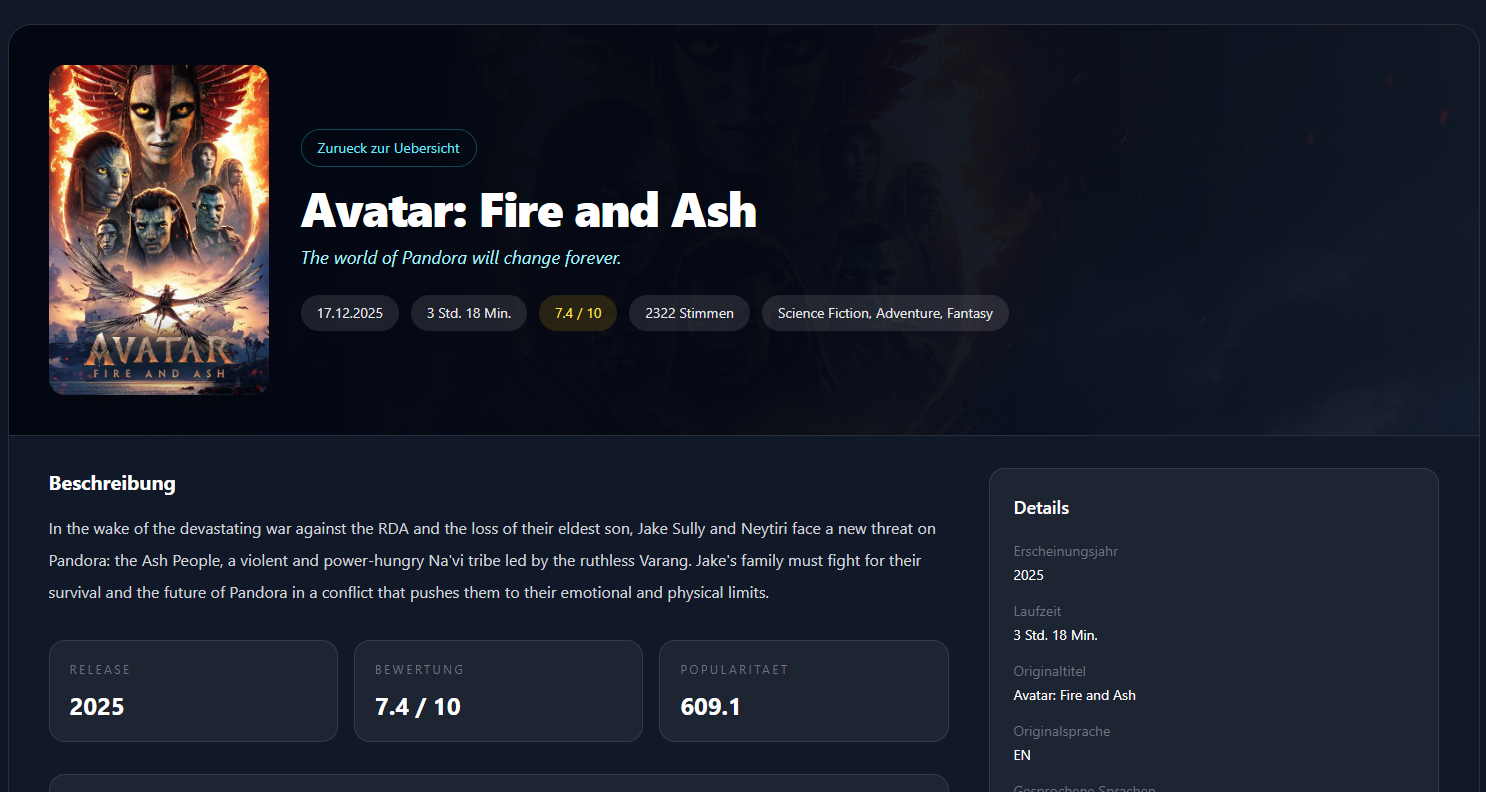
\includegraphics[width=\textwidth]{pics/Abbildung_2_DetailPage}
    \caption{Film-Detailansicht mit Poster, Metadaten und Kurzbeschreibung}
    \label{fig:placeholder_movie_search}
\end{figure}

\begin{figure}[H]
    \centering
    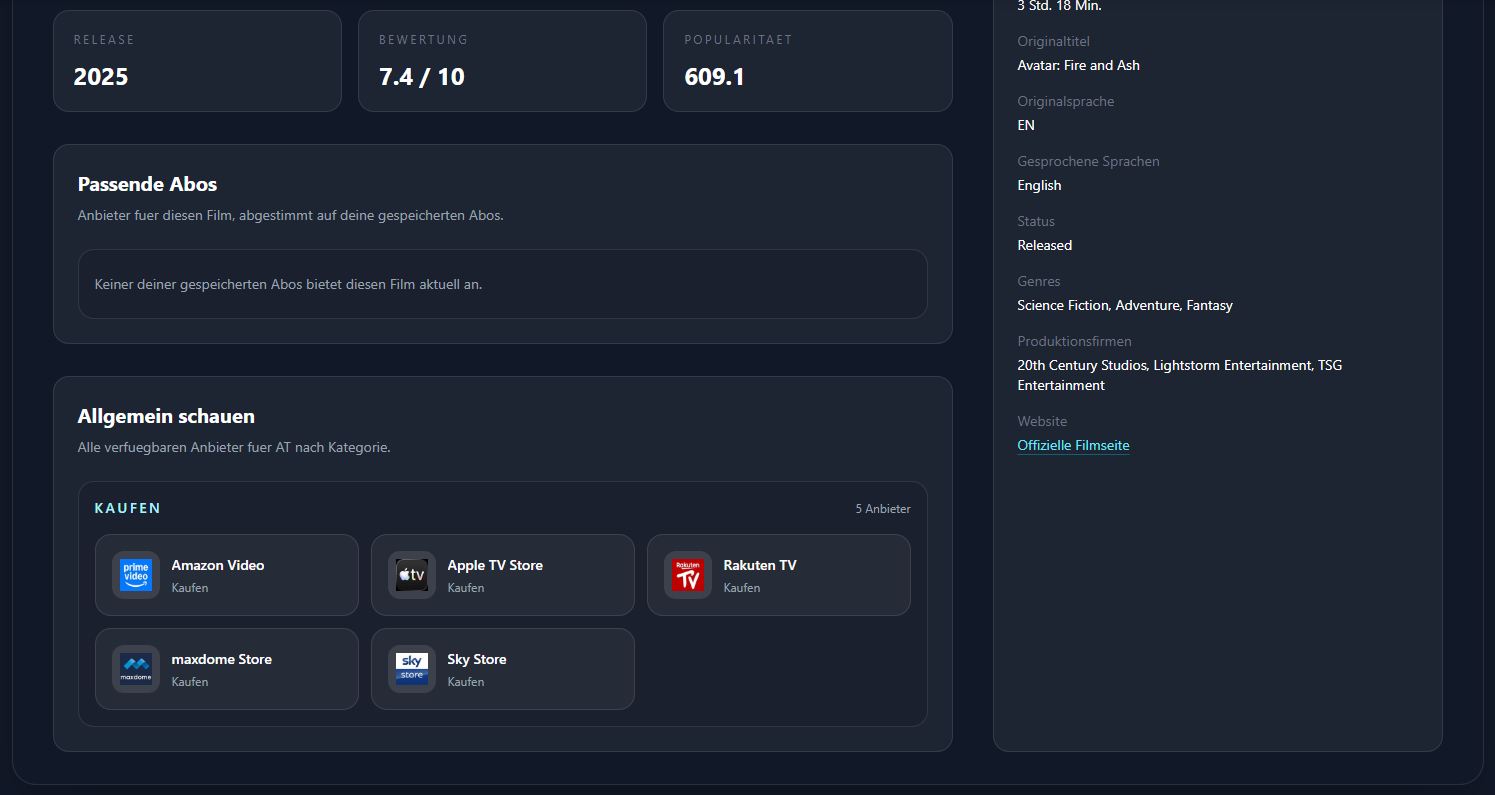
\includegraphics[width=\textwidth]{pics/Abbildung_2_DetailPage_2}
    \caption{Film-Detailansicht mit Abgleich gespeicherter Abonnements und Anbieterübersicht}
    \label{fig:placeholder_movie_detail}
\end{figure}

\section{Account- und Passwortverwaltung}
Die Benutzerverwaltung wurde im Frontend nicht als Eigenlösung umgesetzt, sondern über die Integration von Keycloak realisiert. Dadurch konnte auf eine eigene Passwortspeicherung verzichtet werden, während gleichzeitig ein professioneller und sicherer Anmeldeprozess in die Anwendung eingebunden wurde \cite{keycloak_docs,keycloak_home}. Für meinen Projektteil war vor allem relevant, wie sich Login, Registrierung und geschützte Routen in die Angular-Anwendung integrieren lassen.

\subsection{Einbindung von Login und Registrierung}
Im Frontend wurden Login- und Registrierungsfunktionen so eingebunden, dass Nutzende bei Bedarf an das Keycloak-System weitergeleitet werden. Nach erfolgreicher Anmeldung kehren sie in die Anwendung zurück und können geschützte Bereiche verwenden. Dadurch bleibt der Authentifizierungsprozess klar vom restlichen Frontend getrennt und dennoch benutzerfreundlich in die Anwendung eingebettet.

\subsection{Geschützte Bereiche im Frontend}
Bestimmte Bereiche, insbesondere die Verwaltung persönlicher Abonnements, sind nur für angemeldete Nutzende zugänglich. Das Frontend prüft dafür den Authentifizierungsstatus und steuert den Zugriff auf geschützte Routen. Dadurch wird verhindert, dass persönliche Funktionen ohne gültige Anmeldung aufgerufen werden können. Projektbezogen bedeutete das, dass öffentliche Filmfunktionen und persönliche Verwaltungsansichten bewusst unterschiedlich behandelt wurden: Filmsuche und Detailseiten bleiben offen nutzbar, während die Abo-Verwaltung erst nach erfolgreicher Anmeldung eingebunden wird.

Der Login-Status wirkt sich dabei auch auf die Navigation aus. In der Benutzeroberfläche musste erkennbar sein, ob eine Person bereits angemeldet ist und ob geschützte Menüpunkte verfügbar gemacht werden dürfen. Diese Kopplung zwischen Authentifizierungsstatus und Navigation war ein wichtiger Teil der Frontend-Logik, weil die Anwendung sonst entweder zu viele Funktionen öffentlich anzeigen oder geschützte Bereiche unklar behandeln würde.

\subsection{Verwendung von Bearer-Token bei geschützten Requests}
Ein wichtiger technischer Punkt der Umsetzung war, dass benutzerspezifische Daten nicht ohne Authentifizierung geladen werden können. Wenn das Frontend persönliche Informationen vom Backend anfordert, muss ein gültiges Bearer-Token mitgesendet werden. Dieses Token wird nach erfolgreicher Anmeldung über Keycloak bereitgestellt und bei geschützten HTTP-Anfragen übertragen \cite{keycloak_docs}. Erst dadurch kann das Backend prüfen, ob die anfragende Person berechtigt ist, auf die jeweiligen Daten zuzugreifen.

Für das Projekt war dabei vor allem entscheidend, diese Token-Verwendung nicht in jeder einzelnen Komponente separat zu behandeln. Die Authentifizierungslogik musste zentral organisiert werden, damit geschützte Requests für Abo-Daten, Änderungen und persönliche Anbieterinformationen konsistent verarbeitet werden können. Dadurch blieb die eigentliche Oberflächenlogik schlanker, während die sicherheitsrelevante Weitergabe des Tokens an zentraler Stelle mitgedacht werden konnte.

\subsection{Herausforderungen bei der Integration von Keycloak}
Die Integration von Keycloak in Angular war mit mehreren Herausforderungen verbunden. Dazu gehörten insbesondere die korrekte Weiterleitung nach dem Login, die Behandlung geschützter Routen sowie die sichere Übergabe des Bearer-Tokens bei Anfragen an das Backend. Diese Punkte waren im Frontend besonders relevant, da die Anwendung nur dann benutzerfreundlich funktioniert, wenn Anmeldung, Rückleitung und Zugriffsschutz zuverlässig zusammenspielen. Die Auseinandersetzung mit diesen Problemen war daher ein wichtiger Teil meines praktischen Projektbeitrags.

\subsection{Analyse bestehender Lösungen}
Im Zusammenhang mit Benutzerkonten stellte sich die Frage, ob zusätzlich eine eigene Passwortverwaltung innerhalb der Anwendung umgesetzt werden sollte. Bei der Betrachtung bestehender Lösungen wie Bitwarden oder 1Password wird jedoch deutlich, dass sich professionelle Passwortverwaltung auf Sicherheit, Verschlüsselung und geräteübergreifende Synchronisation spezialisiert \cite{keycloak_home}. Diese Zielsetzung unterscheidet sich klar vom Schwerpunkt des MedienAbonnementManagers.

\subsection{Sicherheits- und Datenschutzbetrachtung}
Eine selbst entwickelte Verwaltung von Passwörtern oder besonders sensiblen Zugangsdaten hätte hohe Anforderungen an Datenschutz und Sicherheit gestellt. Da der Fokus meines Projektteils auf der Frontend-Entwicklung lag, wurde bewusst auf eine eigene Passwortlösung verzichtet. Stattdessen war es sinnvoller, ein bestehendes Authentifizierungssystem einzubinden und die Anwendung auf ihre eigentlichen Kernfunktionen zu konzentrieren. Die Entscheidung zugunsten von Keycloak war damit eine bewusste Abwägung zwischen Funktionsumfang, Sicherheit, Wartbarkeit und verfügbarem Projektzeitraum.

\subsection{Entscheidung: Eigenlösung vs. Integration}
Die Entscheidung fiel daher zugunsten einer Integration von Keycloak und gegen eine selbst entwickelte Passwortverwaltung. Eine Eigenlösung hätte zwar mehr direkten Gestaltungsspielraum geboten, hätte aber gleichzeitig zusätzliche Verantwortung für Passwortspeicherung, Sicherheitsprüfungen und Fehlerbehandlung bedeutet. Die gewählte Integration reduziert die Komplexität im Frontend, verbessert die Sicherheit und ermöglicht eine klarere Trennung zwischen Benutzeroberfläche und Authentifizierungslogik. Für das Projekt war diese Entscheidung sowohl technisch als auch organisatorisch sinnvoll.

\begin{figure}[H]
    \centering
    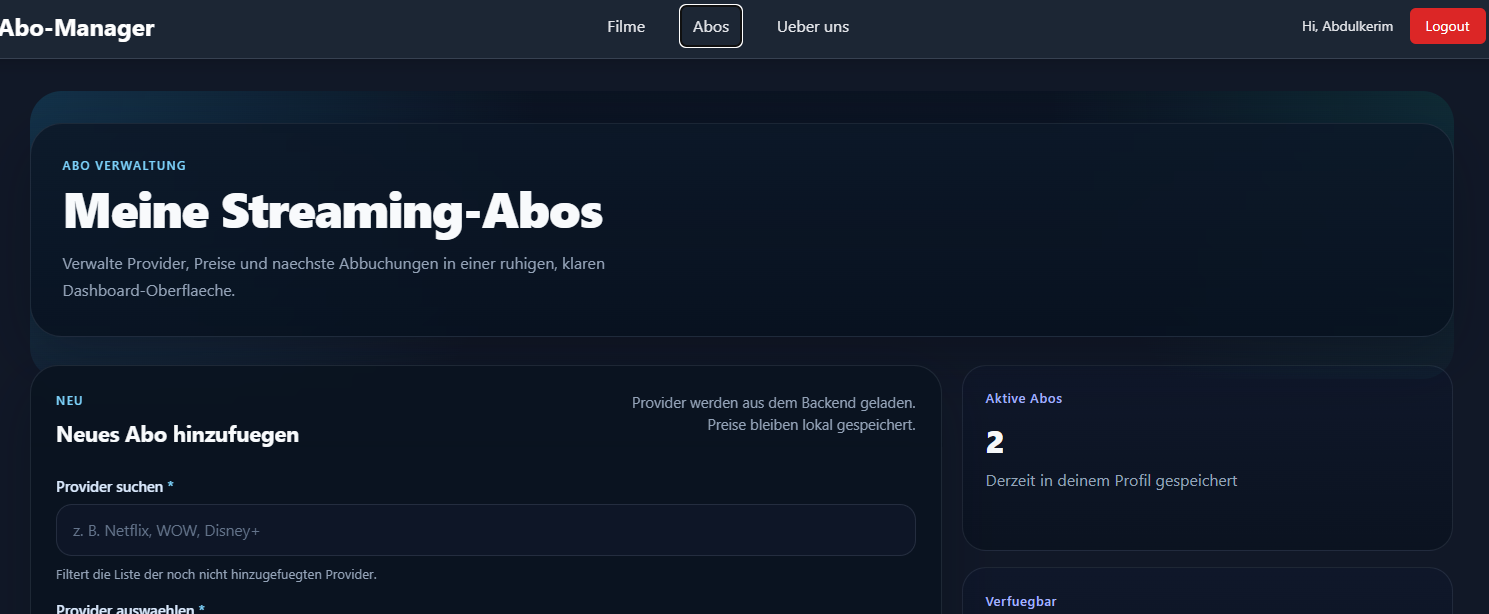
\includegraphics[width=\textwidth]{pics/6.4.7_Bild}
    \caption{Geschützter Bereich der Abo-Verwaltung nach erfolgreicher Anmeldung}
    \label{fig:placeholder_login}
\end{figure}

\section{Herausforderungen und Reflexion der Frontend-Entwicklung}
Im Verlauf der Frontend-Umsetzung zeigte sich, dass nicht nur die reine Darstellung von Oberflächen relevant ist, sondern vor allem die saubere Verbindung zwischen Benutzerführung, Authentifizierung und Datenlogik. Gerade dort entstanden mehrere Erkenntnisse, die für den Projektverlauf und für die eigene fachliche Weiterentwicklung wesentlich waren.

\subsection{Herausforderungen bei der Integration von Keycloak in Angular}
Eine der größten Herausforderungen meines Projektteils war die Integration von Keycloak in das Angular-Frontend. Ein praktisches Problem dabei war, dass für aktuelle Angular-Versionen vergleichsweise wenig gut strukturierte und direkt übertragbare Beispiele verfügbar waren. Viele gefundene Lösungen bezogen sich auf ältere Projektstände, unvollständige Konfigurationen oder andere Framework-Kombinationen. Dadurch war es notwendig, die Einbindung von Login, Redirect, Token-Verwaltung und geschützten Routen schrittweise selbst nachzuvollziehen und an die eigene Anwendung anzupassen.

Ein konkretes Beispiel war die Frage, wann geschützte Inhalte tatsächlich geladen werden dürfen. Die reine erfolgreiche Anmeldung reichte dafür noch nicht aus; zusätzlich musste sichergestellt werden, dass der Rückweg aus dem Login korrekt verarbeitet wird und geschützte Requests erst dann abgesendet werden, wenn der Authentifizierungsstatus und das Token im Frontend wirklich verfügbar sind. Diese Abstimmung zwischen Routing, Login-Rückleitung und Datenabruf war kein rein theoretisches Problem, sondern eine praktische Hürde in der Umsetzung.

\subsection{Herausforderungen bei der Umsetzung von Backend-Daten in der Benutzeroberfläche}
Ein weiterer anspruchsvoller Punkt war die Übersetzung der vom Backend gelieferten Informationen in eine für Nutzende logische und leicht verständliche Oberfläche. Die gelieferten Daten mussten nicht nur technisch korrekt angezeigt, sondern auch sinnvoll gruppiert, gefiltert und mit Interaktionen verknüpft werden. Besonders bei Providerdaten, persönlichen Abonnements und filmbasierten Anbieterinformationen war es wichtig, die Datenstruktur aus Services und DTOs so in die UI zu übertragen, dass die Oberfläche konsistent bleibt und Nutzende die Zusammenhänge schnell erfassen können.

Ein konkretes Beispiel dafür war die Detailansicht eines Films mit Anbieterabgleich. Das Backend liefert einerseits allgemeine Anbieterinformationen zum ausgewählten Film und andererseits benutzerspezifische Abo-Daten. Im Frontend mussten diese beiden Datenquellen so zusammengeführt werden, dass sichtbar wird, welche Anbieter grundsätzlich vorhanden sind und welche davon bereits zum persönlichen Profil gehören. Die Herausforderung lag also nicht nur im Anzeigen der Daten, sondern im sinnvollen Zusammenführen zweier fachlich unterschiedlicher Informationsarten innerhalb derselben Ansicht.

\subsection{Reflexion der anfänglichen Frontend-Entscheidungen}
Rückblickend wurde deutlich, dass eine frühe Oberflächenidee nicht automatisch auch die beste Struktur für die spätere Weiterentwicklung darstellt. Zu Beginn lag der Fokus stark darauf, einzelne Funktionen möglichst schnell sichtbar zu machen. Erst im Verlauf der Umsetzung zeigte sich, wie wichtig eine klare Trennung zwischen Komponenten, Services, Zuständen und geschützten Bereichen ist. Diese Erkenntnis war für die Frontend-Entwicklung ähnlich wertvoll wie die Datenbank-Reflexion im Backend, weil sie gezeigt hat, dass gute Wartbarkeit nicht nur durch funktionierenden Code entsteht, sondern durch eine durchdachte Oberflächen- und Zustandsstruktur. Aus heutiger Sicht würde ich diese Struktur früher festlegen und die Datenflüsse von Beginn an konsequenter entlang fachlicher Verantwortlichkeiten aufteilen.

Ein Beispiel dafür war die anfängliche Tendenz, Datenlogik zu nah an sichtbaren Komponenten zu behandeln. Solange einzelne Ansichten noch klein waren, funktionierte dieser pragmatische Ansatz, mit wachsender Komplexität bei Suche, Detaildarstellung und Abo-Verwaltung wurde er jedoch unübersichtlicher. Erst die stärkere Verlagerung von Request-Logik und Datenverarbeitung in Services machte die Oberfläche langfristig wartbarer.

\subsection{Erkenntnisgewinn für den weiteren Projektverlauf}
Die Auseinandersetzung mit diesen Frontend-Problemen hat wesentlich dazu beigetragen, die Anwendung systematischer weiterzuentwickeln. Insbesondere die Keycloak-Integration und die saubere Abbildung von Backend-Daten auf UI-Komponenten haben gezeigt, dass moderne Webentwicklung nicht nur aus Design und API-Aufrufen besteht, sondern ein durchgängiges Verständnis von Authentifizierung, Datenfluss und Benutzerführung erfordert. Gerade dieser Lernprozess stellt einen wichtigen Teil meines persönlichen Beitrags zur Diplomarbeit dar.
